\documentclass[12pt,a4paper]{article}
\usepackage{ssn-be-cse-review}
\usepackage{float}
\usepackage{url}
\usepackage{alltt}
\usepackage{subcaption} 
\usepackage{longtable}
%\usepackage{mathtools}
\usepackage{algorithm2e}[1]
\usepackage{tikz}
\usetikzlibrary{shapes,arrows}
\usetikzlibrary{trees}
\usepackage{amsmath}
\documentclass{article}
\usepackage{graphicx}
\usepackage[colorlinks=true,linkcolor=black,citecolor=black]{hyperref}
\graphicspath{ {./images/} }


\begin{document}
   
\ptitle{Person Identification using Gait Analysis}
\review{1}
\setnauthors{4}
\setauthorone{Siddharth S}{205001106}
\setauthortwo{Rahul Rajagopalan}{205001081}
\semester{8}
\guide{Dr Sakaya Milton R}
\reviewdate{9,10 February 2024}
\reviewtitle
\hrule

\section{Introduction}

\subsection{Background}
Person identification using gait analysis is a promising tool to enhance security, especially in settings like airports, secure facilities, and online accounts where safeguarding identities and data is vital. It provides a non-intrusive and reliable biometric authentication method, making it challenging for impostors to access personal information, thereby reducing identity theft and protecting individuals from financial and personal losses. Additionally, it can significantly aid law enforcement agencies in identifying and tracking suspects, potentially leading to quicker resolutions of criminal cases and enhancing public safety.

\subsection{Purpose}
The project aims to develop a machine learning model capable of efficiently identifying individuals even while considering additional factors such as bags and clothing. This enhances the overall person identification accuracy.

\subsection{Scope of the project}
Previous studies in gait analysis for person identification have achieved good accuracy under carrying conditions but struggled to deliver satisfactory results in clothing conditions. Furthermore, the use of unsupervised image-to-image translation GANs in this context is limited. Hence, our goal is to utilize three GAN models, DiscoGAN, CycleWGAN and our novel approach ,M-DiscoGAN, and subject the output images to a voting classifier, to improve the accuracy. In doing so, we aim to address the challenges associated with clothing conditions and enhance the overall performance of gait analysis for person identification.

\subsection{Proposed method overview}
The project involves a three-step process: first, individual frames are transformed into Gait Energy Images (GEIs). These GEIs capture the walking patterns of individuals with or without the covariate factors such as bags or clothes. These images are then fed into the model, which generates GEIs without the covariate factors. Finally, the translated images are passed through a Convolutional Neural Network (CNN) for person identification.

\subsection{Expected outcomes}
 The current method for person identification through gait analysis relies on CycleGAN, achieving an accuracy of 79\% for subjects carrying objects and 52\% for subjects with varying clothing. This new approach is expected to achieve better results than the already existing model.

% \section{Problem statement}

% Person identification using gait analysis is a challenging task with critical applications in security, surveillance, and biometrics. The current state of the art offers reliable identification under normal walking conditions, but it encounters significant limitations when individuals exhibit variations in their walking patterns due to covariate factors, such as changes in clothing or carrying objects. , hampering their effectiveness in practical scenarios. Our goal is to develop a novel architecture for a person identification system that can reliably distinguish individuals under various covariate conditions, including different clothing styles and carrying objects

% Our project  focuses on leveraging DiscoGAN and WGAN techniques to achieve the goal of accurately identifying individuals who are wearing various types of overcoats and headcaps or carrying bags. We employ image-to-image translation to eliminate the effects of these accessories and subsequently conduct person identification. To optimize our approach, we integrate the outcomes using a voting classifier. The core objective is to develop a robust system for recognizing people in diverse attire, enhancing security and surveillance applications. 

% \section{Justification for the problem formulation}
% Previous studies in gait analysis for person identification have achieved good accuracy under carrying conditions but struggled to deliver satisfactory results in clothing conditions. Furthermore, the use of unsupervised image-to-image translation GANs in this context is limited. Hence, our goal is to utilize three GAN models, DiscoGAN, CycleWGAN and our novel approach ,M-DiscoGAN, and subject the output images to a voting classifier, to improve the accuracy. In doing so, we aim to address the challenges associated with clothing conditions and enhance the overall performance of gait analysis for person identification.

\section{Literature survey}
Gait analysis offers a dynamic, real-time means of recognizing individuals, making it particularly valuable in security applications. In this context, Generative Adversarial Networks (GANs) have gained attention for their capacity to capture and synthesize realistic gait patterns. A Generative Adversarial Network (GAN) is a deep learning framework consisting of two neural networks: a generator and a discriminator. The generator's role is to create synthetic data, such as images, from random noise. It aims to generate data that is indistinguishable from real data. On the other hand, the discriminator acts as a binary classifier, distinguishing between real data and data produced by the generator. The two networks are in a constant adversarial game, with the generator striving to improve its ability to deceive the discriminator, and the discriminator trying to become better at telling real from fake data. This adversarial process continues until the generator produces data that is extremely realistic.
% \newline
% The cycle consistency loss is given by:
% \begin{align}
%     L_{cyc}(G, F) = E_{a\sim p\setstretch{1}da\setstretch{1}ta(a)}[||F(G(a))-a||_1] + E_{b\sim p\setstretch{1}da\setstretch{1}ta(b)}[||F(G(b))-b||_1]
% \end{align}

% \begin{align}
%     L(G, F, D_A, D_B) = L_{GAN}(G, D_B, A, B) + L_{GAN}(F, D_A, B, A) + \lambda L_{cyc}(G, F)
% \end{align}

Zou et al. \cite{zou2020}, explored the application of deep learning techniques for gait pattern recognition using smartphone sensors, specifically accelerometers and gyroscopes. To distinguish between walking and non-walking data, the methodology incorporates semantic segmentation with a one-dimensional Deep Convolutional Neural Network (DCNN). Gait data is initially transformed into six-axis inertial data, which is then processed through DCNN and Long Short-Term Memory (LSTM) networks to capture spatial and temporal features. Classification is subsequently performed using a Convolutional Neural Network (CNN). The study draws upon the whuGAIT dataset and reports an accuracy of 90.22\% for the classification of walking and non-walking data. However, the research acknowledges certain limitations related to its applicability to individuals with physical impairments and its assumption of consistent smartphone usage.

Manssor et al. \cite{manssor2021}, proposed an improvement in  real-time human recognition under nighttime conditions by integrating the analysis of both facial and gait features. To achieve this, the methodology employs thermal cameras, image normalization techniques, and the YOLOv3 network for the fusion of face and gait classifiers to enhance recognition capabilities. The DHU Night dataset serves as the basis for the study, and it reports notable achievements in recognition rates, with examples including 95.83\% accuracy for lower body angles and 96.50\% when combining upper and lower body angles for analysis.

 Huynh et al.\cite{huynh2020}, advocated a novel approach for person identification through the utilization of 3D spatiotemporal gait features acquired via a convolutional network. The methodology involves the collection of 3D human skeleton data and the subsequent extraction of hierarchical spatiotemporal features. These extracted features serve as the basis for training a Deep Convolutional Neural Network (DCNN) tailored for person identification. The research draws upon several datasets, including UPCV Gait, UPCV Gait K2, KS20 VisLab Multi-View Kinect Skeleton, and SDUGait, and demonstrates impressive accuracy rates, such as 99.65\% for UPCV Gait K2.

Asif et al \cite{asif2022},proposed to facilitate the recognition of human gait patterns in a multi-view setting, accounting for various covariate factors. The methodology hinges on gait images that encompass normal walking conditions, as well as instances of walking with altered clothing and carrying bags. Feature extraction is carried out through Histogram of Oriented Gradients (HOG), and the model employs Support Vector Machine (SVM) classifiers for training and classification. The research relies on the CASIA-B dataset and reports notable achievements in accuracy, such as 87.90\% accuracy for gait recognition when individuals are wearing coats.

 Vasudevan et al.\cite{vasudevan2023}, proposed a gait image classification for medical diagnosis, employing deep learning models and assessing their comparative effectiveness. The methodology encompasses the use of silhouette image data, with feature extraction conducted through OpenCV, and data augmentation when necessary. Gait silhouette images are classified using Convolutional Neural Network (CNN) and a CNN Long Short-Term Memory Network (CNN-LSTM) model. Additionally, the research explores the application of transfer learning models, including MobileNetV2, InceptionV3, VGG16, VGG19, ResNet9, and ResNet50. The datasets employed are CASIA-B and CASIA C. The results highlight the impressive performance of the CNN model, achieving an accuracy of 94.29\%. The study acknowledges certain limitations, especially when dealing with gait variations across different walking angles.

Wen et al.\cite{wen2022}, proposed a study to extract invariant features while retaining individual identity information, particularly in the presence of view transformations using Generative Adversarial Networks (GANs). The methodology involves the utilization of GANs to seamlessly transform gait images across various states and angles into a standardized perspective, incorporating angles of 54°, 90°, and 126°. Subsequently, the study meticulously constructs a multi-view gait recognition model founded on deep convolutional networks, with the final decision model being the K-Nearest Neighbors (KNN) algorithm. This innovative approach enables gait images captured from diverse angles and conditions to be converted into target images, depicting individuals in a standard pose without any accompanying objects. To enhance feature extraction and minimize feature loss, the generator incorporates a residual structure. The fusion of multi-view gait features adeptly mitigates the impact of variations in carrying objects and clothing on recognition accuracy, leading to a substantial boost in the model's performance, especially for sequences involving bags and coats. The evaluation is based on the CASIA-B dataset, yielding recognition accuracy rates of 77.84\% and 50.37\% for gait sequences involving bags and coats, respectively.

Khan et al.\cite{khan2023}, introduced a system for human gait recognition for biometric applications, which is accomplished through the application of Bayesian optimization and the utilization of extreme learning machines (ELM). The research begins by extracting motion regions through optical flow in the initial data processing phase. Subsequently, two distinct models are trained: one model utilizes the extracted motion regions, and the other relies on enhanced video frames, both based on the EfficientNet-B0 architecture. To further enhance model performance, Bayesian optimization is employed to dynamically select hyperparameters during the training process, leading to the creation of two models—one based on motion frames and the other on enhanced frames. In the fusion phase, features are extracted from both models, and a novel parallel fusion technique called Sq-Parallel Fusion (SqPF) is introduced to effectively amalgamate these features. Moreover, an enhanced version of the Tiger optimization algorithm, termed Entropy Variance controlled Tiger optimization (EVcTO), is incorporated into the research. The most discriminative features selected through this process are subsequently classified using an extreme learning machine (ELM) classifier. For evaluation, the experiment leverages two publicly available datasets, CASIA B and CASIA C, achieving an average accuracy of 92.04\% and 94.97\%, respectively.However, the study acknowledges specific limitations. While the fusion of bidirectional information enhances accuracy, it introduces the potential for redundant information. 

Liao et al.\cite{liao2020}, put forth a model-based approach for gait recognition, integrating body pose and human prior knowledge. The methodology initiates with the transformation of 2D pose data into a 3D format, enabling comprehensive analysis of temporal and spatial features. This approach, known as PoseGait, employs Convolutional Neural Networks (CNNs) to estimate human 3D pose from images, enhancing feature extraction for gait recognition. Four distinct feature types (fpose, fangle, flimb, and fmotion) are concatenated at the input level and serve as input for a CNN model responsible for feature extraction. During training, the study employs two loss functions to collectively minimize intra-class variation and enhance inter-class variation. CASIA-B and CASIA-E datasets are used, and the results highlight the method's effectiveness, achieving state-of-the-art performance and robustness against variations in viewing angles and clothing conditions.

Kim et al.\cite{kim2017}, introduced an alternative method for unpaired image-to-image translation called DiscoGAN, short for "Discover Cross-Domain Relations with GAN." Unlike CycleGAN, which emphasizes cycle consistency loss, DiscoGAN is designed to find meaningful cross-domain relationships by utilizing reconstruction losses.It was primarily used to convert edge to photos, style transfers and face conversions.In DiscoGAN, the reconstruction loss is a key component. It measures the dissimilarity between the original image A and the image reconstructed after being sequentially passed through both generators (A-B-A). Two reconstruction losses are computed, one for each generator, typically using the L2 norm (MSE) for loss calculation. This approach provides a more versatile way to handle image-to-image translation tasks, facilitating the discovery of cross-domain relations. The advantage of DiscoGAN is that the main essence of the image is kept intact and only necessary factors are changed.

% \begin{align}
%     x_{AB} = G_{AB}(x_A)
% \end{align}
% \begin{align}
%     x_{ABA} = G_{BA}(x_{AB}) = G_{BA}.G_{AB}(x_A)
% \end{align}
% \begin{align}
%     L_{reconst_A} = d(G_{BA}.G_{AB}(x_A), x_A)
% \end{align}
% \begin{align}
%     L_{GAN_B} = -E_{x_A\sim p_A}[logD_B(G_{AB}(x_A))]
% \end{align}
% \begin{align}
%     L_{G_{AB}} = L_{GAN_B} + L_{reconst_A}
% \end{align}
Martin Arjovskyet et al. \cite{arjovsky2017} and Hu et al.\cite{hu2021}, introduced a groundbreaking variant of Generative Adversarial Networks (GANs) that addresses several critical challenges in GAN training. Traditional GANs struggle with issues like mode collapse, vanishing/exploding gradients, and the absence of a meaningful loss function. Wasserstein-GAN (WGAN) tackles these problems by introducing the Wasserstein distance, also known as the Earth Mover's (EM) distance, as a novel loss function. The Wasserstein distance offers a more intuitive and stable way to measure the "distance" between probability distributions, making it a superior choice for evaluating GANs. WGAN also introduces the concept of a Lipschitz constraint on the critic (discriminator) network, aiming to ensure that it does not produce extreme gradients, which can lead to instability in training. Rather than relying on weight clipping, WGAN employs a "gradient penalty" approach to enforce the Lipschitz constraint.

Zhu et al., \cite{zhu2017}, introduced the innovative CycleGAN concept and framework. CycleGAN represents a novel approach for image-to-image translation that doesn't rely on paired datasets.It leverages a cycle-consistency loss to ensure that translated images are coherent in both directions, making it particularly useful for tasks like style transfer, object transfiguration, and more. CycleGAN is designed as a generic image translation framework and may not be the best choice for domain-specific applications. In such cases, specialized models might perform better. 

Alsaggaf et al.,\cite{alsaggaf2021} introduced a paper that addresses the challenges of identifying individuals with normal walking patterns in uncooperative environments. It employs a Cycle Consistent Generative Adversarial Network (CCGAN) to transform Gait Energy Images (GEIs) that have been disturbed by various factors back to their normal states. The method operates as an unsupervised learning process where GEIs affected by different covariate factors act as the source domain, and the goal is to translate them to the target domain, representing the undisturbed walking conditions. Using the Cycle Loss function, the CCGANs automatically establish pairs of GEIs for individuals and generate the necessary transformations. These pairs are subsequently evaluated by a Convolutional Neural Network (CNN) model to predict the person's identity.The proposed method removes the covariate factors such as bags and clothes, and achieves an accuracy score of 79\% in carrying conditions and 52\% in clothing conditions. This proposed method does not perform well in clothing conditions.
\newline
\newline


\section{Feasibility Study}
Our project on gait analysis introduces a feasible and novel approach. We have access to an existing dataset, CASIA-B which contains Gait Energy Image (GEIs) of 124 subjects with each subject consisting of 6 normal walk conditions, 2 carrying conditions, and 2 clothing conditions.  Each condition has over 50 images from 10 different angles. It has a total of 19139 images. With the existing dataset and by utilizing existing platforms like Colab or Kaggle, we ensure that the implementation of the project is feasible. The project's scalability is a key strength, as it can be potentially extended to real-time surveillance applications. All these factors collectively make our project feasible.


% In practical terms, WGAN enhances the training stability and convergence of GANs, resulting in more reliable generation of high-quality samples. It is a theoretical and practical breakthrough in the field of generative models, providing a rigorous mathematical framework through the Wasserstein distance, thus significantly advancing our understanding of GANs.



% \begin{aligned}
% L_{WGANGP}(G, D_B, A, B) =   E_{b\sim{p_{data}}(b)}[D_B(b)]  -  E_{a\sim{p_{data}}(a)}[D_B(G(a))]  + \\
% \lambda_{gp} \cdot E_{c\sim{p_{in.dist.}}(c)}[(|\nabla_c D_B(c)|_2 - 1)^2]
% \end{aligned}

% \begin{aligned}
% L(G, F, D_A, D_B)  =  L_{WGANGP}(G, D_B, A, B)   + \\
% L_{WGANGP}(F, D_A, A, B)   + \\
% \lambda_{c} \cdot L_{cyc}(G,F)   + \\
% \lambda_{i} \cdot L_{identity}(G, F)
% \end{aligned}


% Various approaches leverage a range of Generative Adversarial Networks (GANs) to facilitate image-to-image conversion across different domains. Among these methods, CycleGAN stands out as it enables unpaired image translation.  These approaches encompass both paired and unpaired image-to-image translation. Paired techniques necessitate meticulously curated datasets, which are often impractical in real-time scenarios, underscoring the practicality of unpaired methods.  The seminal work, "Unpaired Image-to-Image Translation Using Cycle-Consistent Adversarial Networks" authored by Jun-Yan Zhu, Taesung Park, Phillip Isola, and Alexei A. Efros[6], introduced the innovative CycleGAN concept and framework. CycleGAN represents a novel approach for image-to-image translation that doesn't rely on paired datasets. 
% \newline
% \newline
%  This paper introduces CycleGAN, a novel approach for image-to-image translation without requiring paired data. It leverages a cycle-consistency loss to ensure that translated images are coherent in both directions, making it particularly useful for tasks like style transfer, object transfiguration, and more. CycleGAN is designed as a generic image translation framework and may not be the best choice for domain-specific applications. In such cases, specialized models might perform better. 
% \newline
% \newline
% Another approach involves the use of CCGAN[1]. One of the distinguishing features of CCGANs is the emphasis on a continuous latent space. This means that small changes in the noise vector or condition vector should result in gradual and visually coherent changes in the generated images. This allows for more fine-grained control over the generated content.
% \newline
% \newline
% Other GAN techniques, such as DiscoGAN[2], WGAN[4], DualGAN[3], etc have shown superior performance in various applications. We aim to combine the performance DiscoGAN and WGAN using a voting classifier to fully optimize our model.

 
 





\section{Proposed system}

Surveillance cameras capture continuous video streams that are first processed frame by frame. Each frame represents a snapshot in time and contains information about the individuals within the camera's field of view. These frames serve as the initial data source for the subsequent stages of the system.

To capture the unique walking patterns of individuals, the frames are transformed into Gait Energy Images (GEIs). These GEIs are essentially silhouette images that focus solely on the individual's body shape and gait, eliminating any extraneous details. The creation of GEIs is a crucial step as it reduces the complexity of the images and highlights the distinctive characteristics of each person's gait.

\begin{figure}[!h]
  \centering
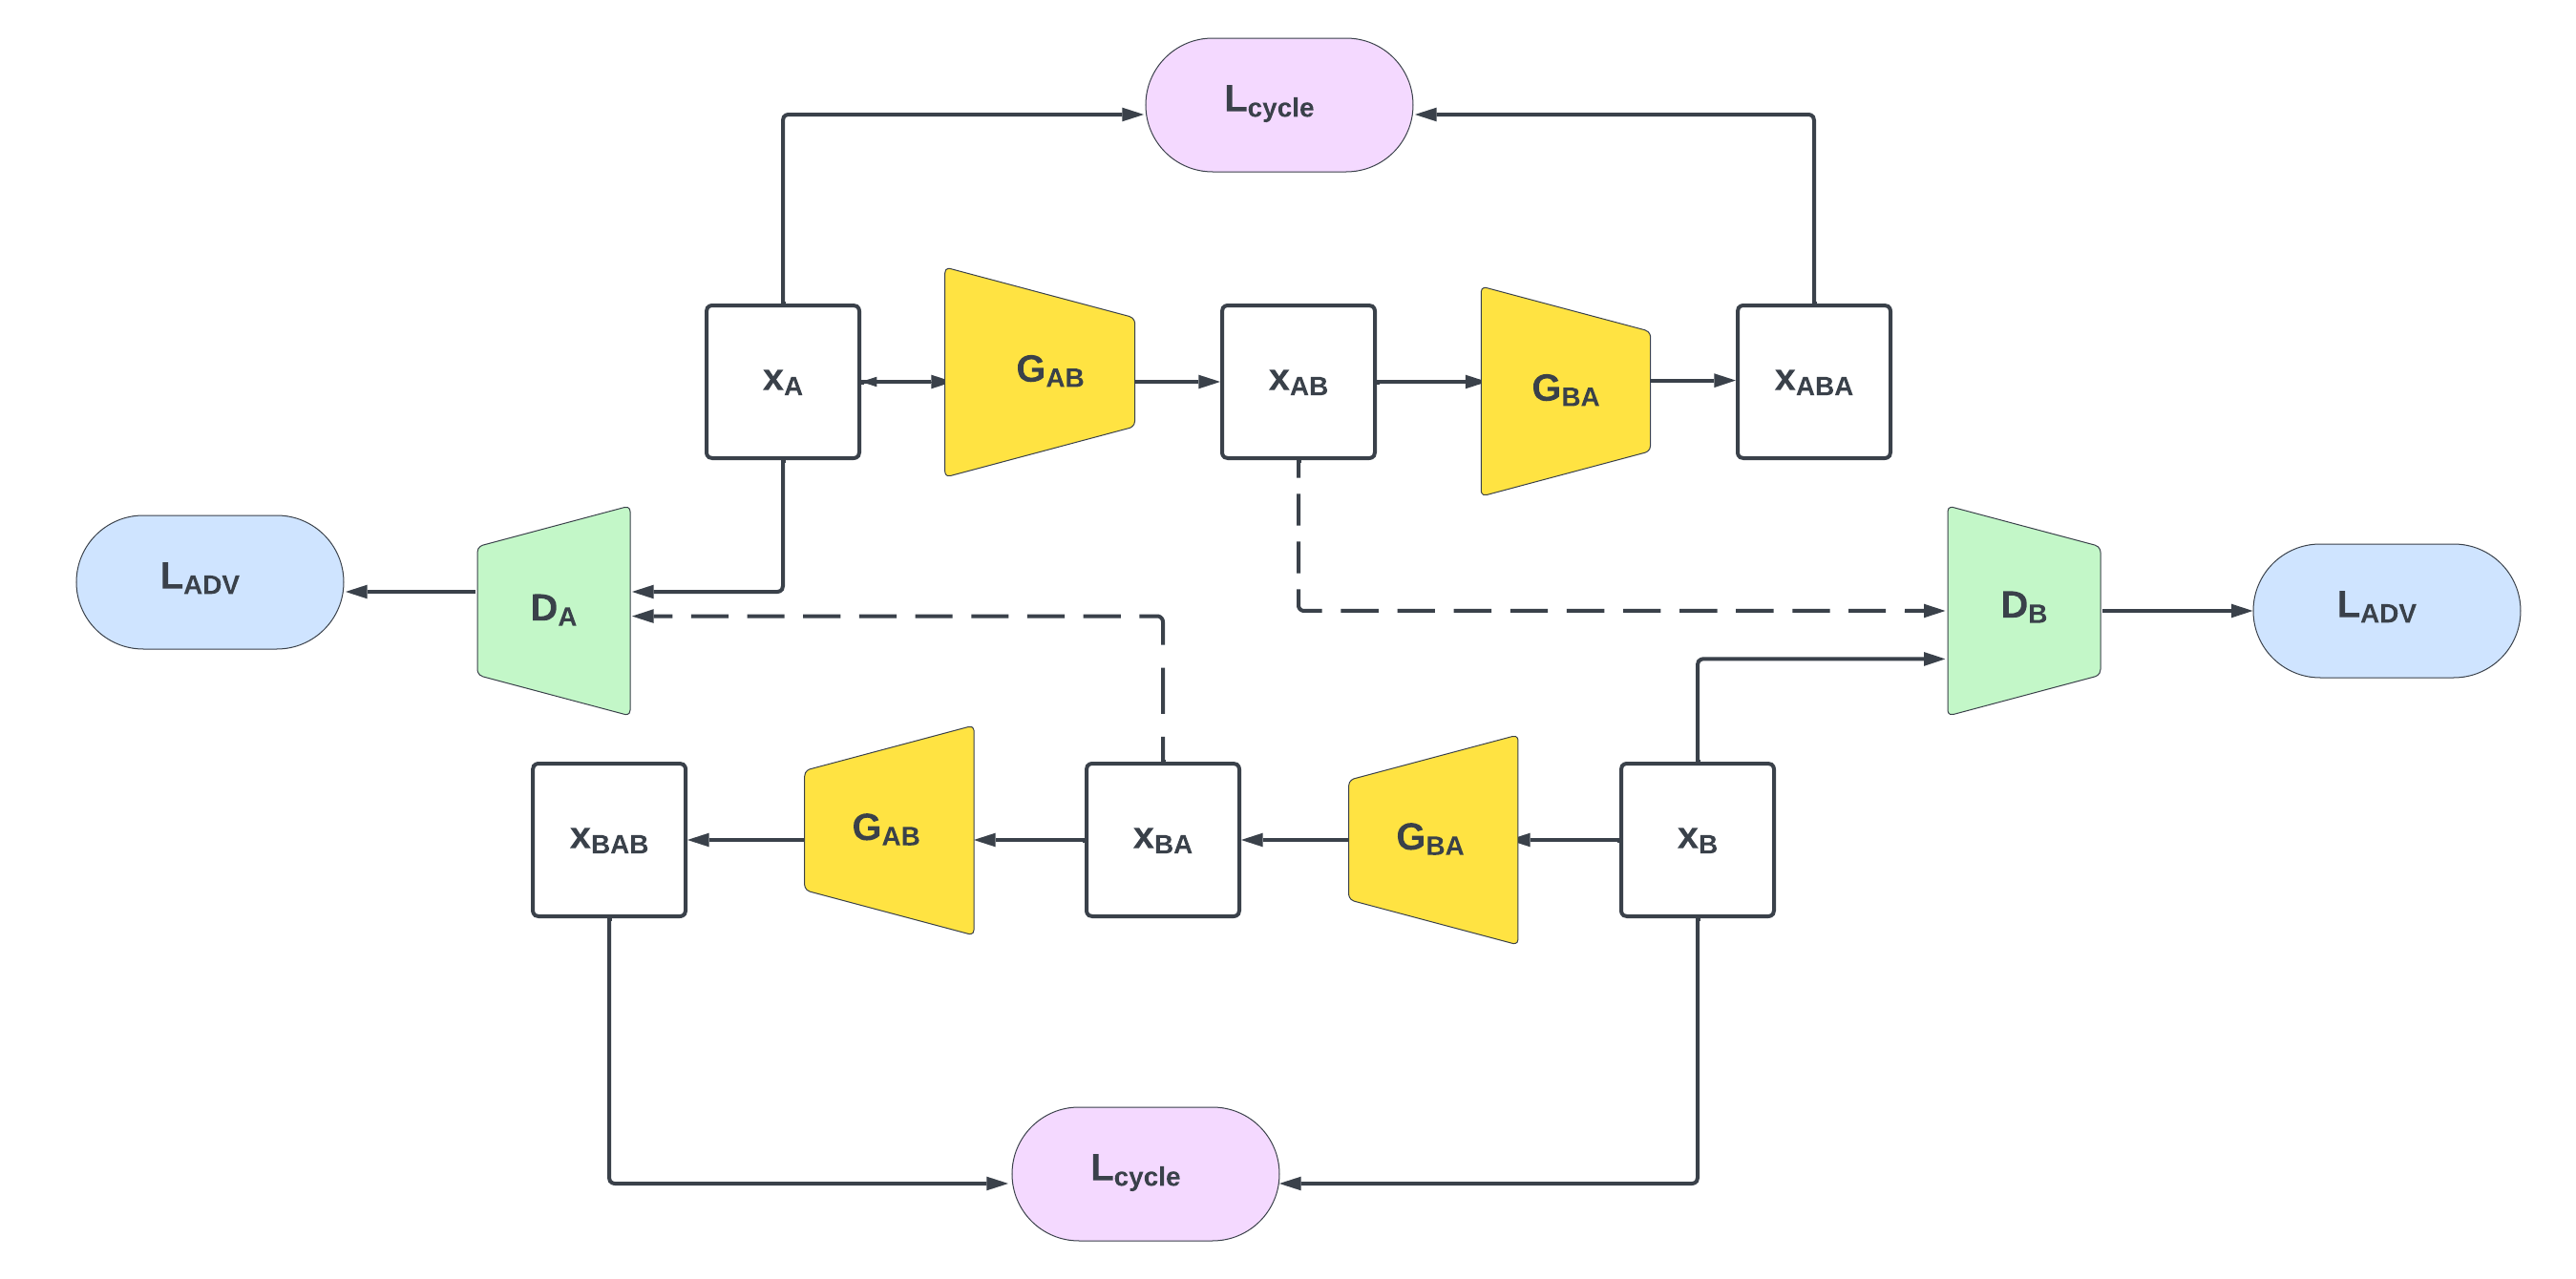
\includegraphics[scale=0.4]{images/color-cc.png}
  \caption{The Existing framework using CycleGAN}
  \label{fig:Overall}
\end{figure}

The existing structure uses a cycleGAN architecture. $x_A$ represents the real input image in domain A. It is passed through $G_{AB}$ which is a generator that converts image from domain A to B. The generated fake image in domain B is labeled as $x_{AB}$. This is then passed through another generator $G_{BA}$, which converts it back to an image from domain A.
This is labeled as $x_{ABA}$. The fake and the real images of each domain are passed through discriminators, $D_A$ and $D_B$ respectively. $L_{ADV}$ represents the adversarial loss, which is calculated based on the comparison between the fake and the real image. The real images and the reconstructed images in both domains are compared and the cycle loss $L_{cycle}$ is calculated. A similar process happens for $x_B$ when passed through the respective generators and discriminators.
\newline

\begin{figure}[!h]
  \centering
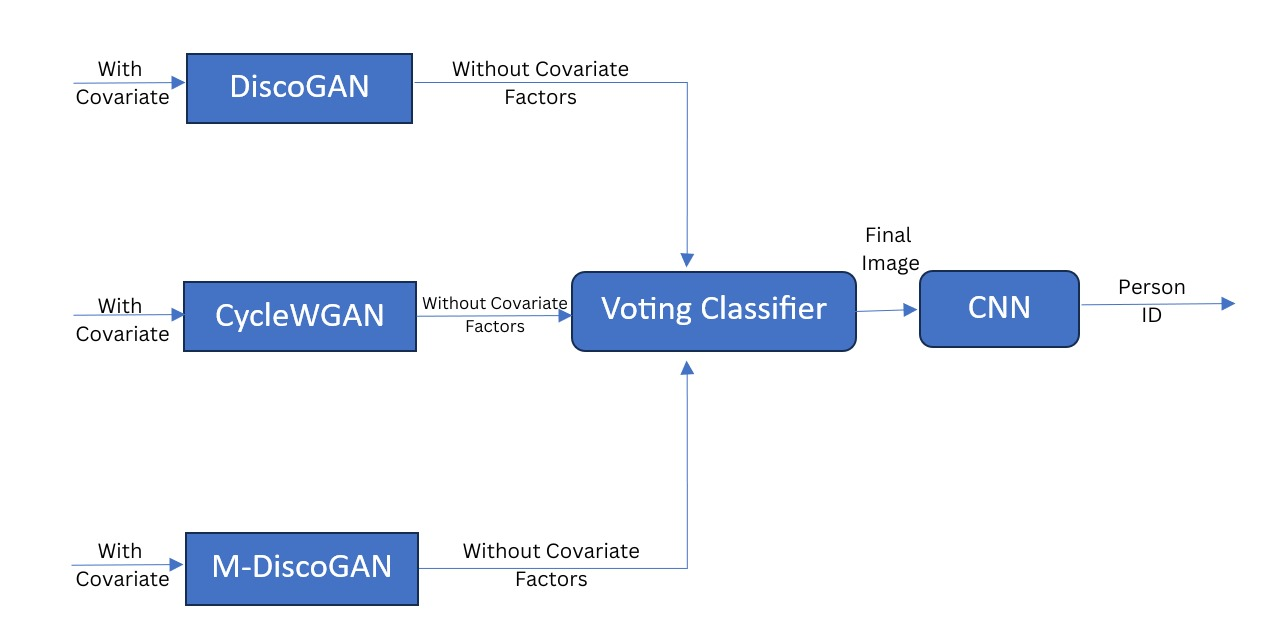
\includegraphics[scale=0.5]{images/overall.jpg}
  \caption{The proposed framework for person identification using gait analysis}
  \label{fig:Overall}
\end{figure}

The model that we propose leverages three distinct unsupervised image-to-image translation techniques: DiscoGAN, CycleWGAN, and M-DiscoGAN. These models transform input GEI images simultaneously and they each generate an output image. To further enhance the quality and reliability of the final image, the outputs from models are subjected to a voting classifier, which aggregates their results. The combined output is then channeled through a Convolutional Neural Network (CNN) layer, where person identification takes place. This comprehensive approach ensures that the final image not only benefits from the strengths of the image translation models but also undergoes an additional layer of processing to refine and solidify the identification process.

\clearpage
\subsection{Cycle wGAN}
\begin{figure}[!h]
  \centering
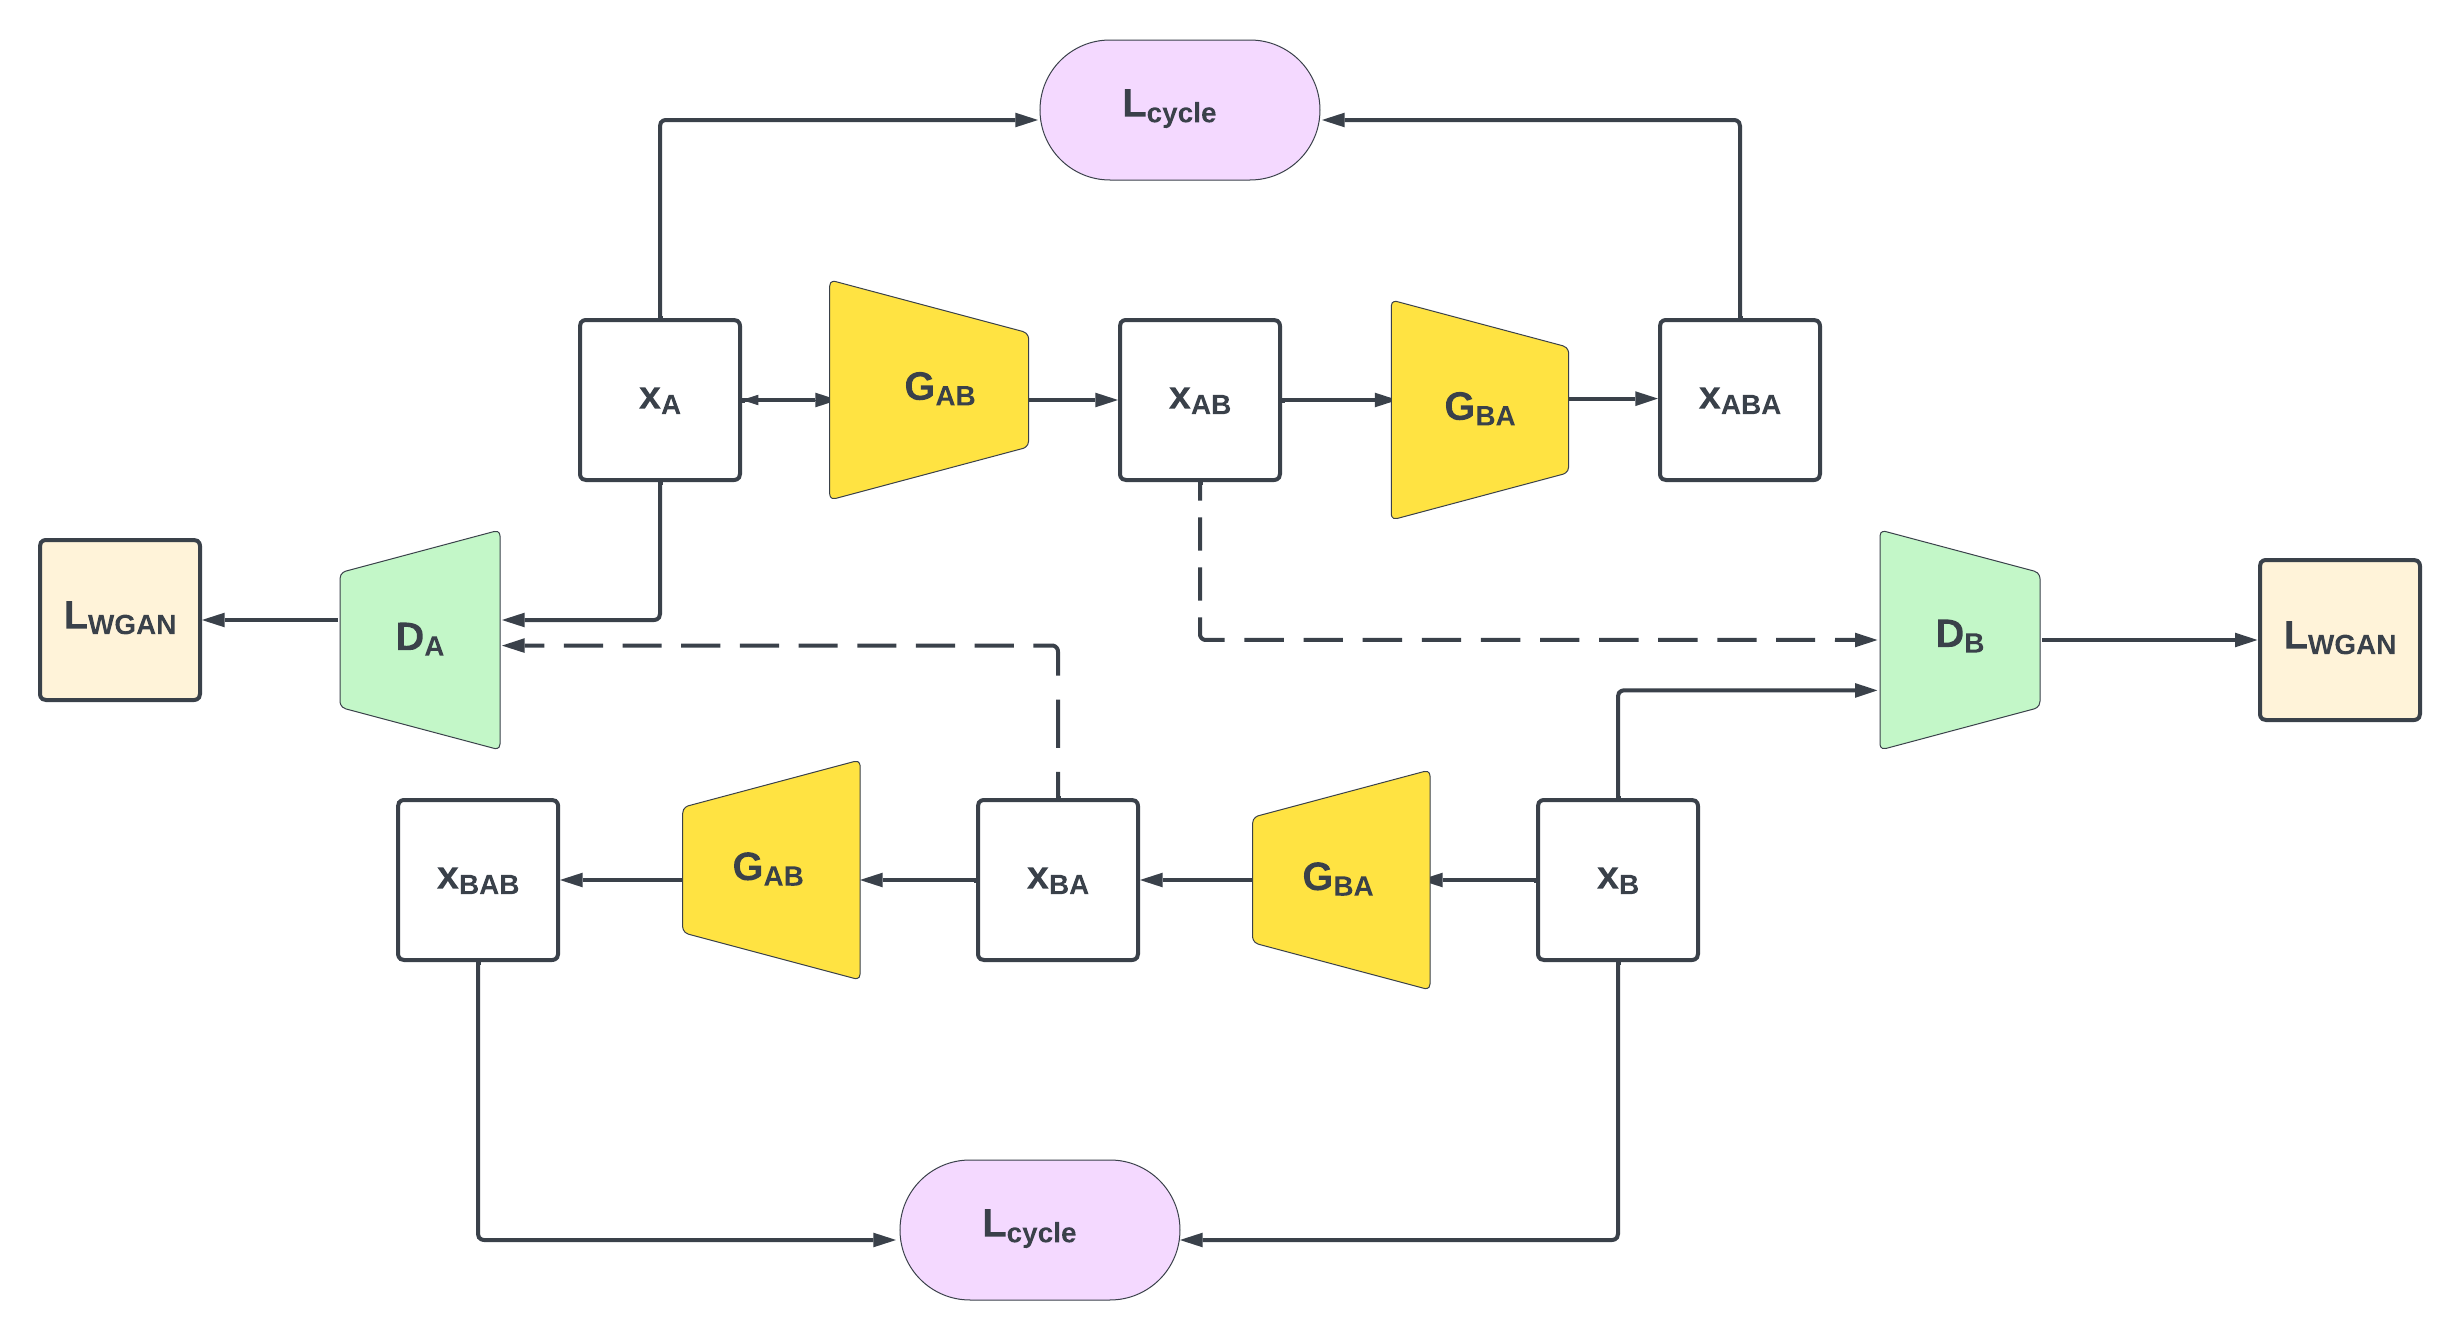
\includegraphics[scale = 0.4]{images/color_cw.png}
  \caption{cycleWGAN Architecture}
  \label{fig:cycleWGAN}
\end{figure}

The architecture follows the basic CycleGAN architecture. 
The input image, with the covariate factors, is passed through generator AB that removes the covariate factors and converts it into a normal image of domain B. This image is then passed to generator BA that adds the covariate factors to convert it back to domain A. The original image and this image are evaluated and the cycle loss is computed. The two discriminators/critics of the respective generators take the input image and the cross domain generated image and calculates the Wasserstein loss which compares the distribution of the real and fake images. The discriminator assigns a higher score to the real image and a lower score to the fake image. Apart from this, the input image is passed through the generator of the other domain to calculate the identity loss. This is done to retain the features of the input image.
$x_A$ and $x_B$ represent the input data in the two domains. $G_{AB}$ and $G_{BA}$ represent the the generators of the two domains while $D_A$ and $D_B$ are the discriminators. $x_{AB}$ and $x_{BA}$ are the generator-converted fake images. $x_{ABA}$ and $x_{BAB}$ are the reconstructed images. $L_{cycle}$  represents the cycle loss functions. Finally, $L_{WGAN}$ represents the Wasserstein Loss function.

Since the adversarial loss in CycleGANs uses a min-max setup, CycleGANs themselves often face the GAN optimization setbacks. Mode collapse is one of such setbacks, where the generator model learns to create only a single or a small set of outputs.The Wasserstein loss soft constrained by the gradient penatly is defined as:
\newline
\newline
\begin{aligned}
L_{WGANGP}(G, D_B, A, B) =   E_{b\sim{p_{data}}(b)}[D_B(b)]  -  E_{a\sim{p_{data}}(a)}[D_B(G(a))]  + \\
\lambda_{gp} \cdot E_{c\sim{p_{in.dist.}}(c)}[(|\nabla_c D_B(c)|_2 - 1)^2]
\end{aligned}
\newline
\newline
 This equation  represents a random linearly interpolated distribution between the source data distribution  and the target data distribution, helping to avoid mode collapse. Cycle-WGAN models replace the min-max adversarial setup of the CycleGAN's generator and discriminator networks with WGANs.


\subsection{DiscoGAN}
DiscoGAN, short for "Discover Cross-Domain Relations with GAN," is a deep learning architecture designed to facilitate cross-domain image translation, by uncovering meaningful relationships. While CycleGAN emphasizes the preservation of cycle consistency, DiscoGAN concentrates on discovering the cross-domain relations via reconstruction losses. This enables a more versatile and exploratory approach to image-to-image translation tasks, as each generator trains on the losses of its own rather than the total loss.

\begin{figure}[!h]
  \centering
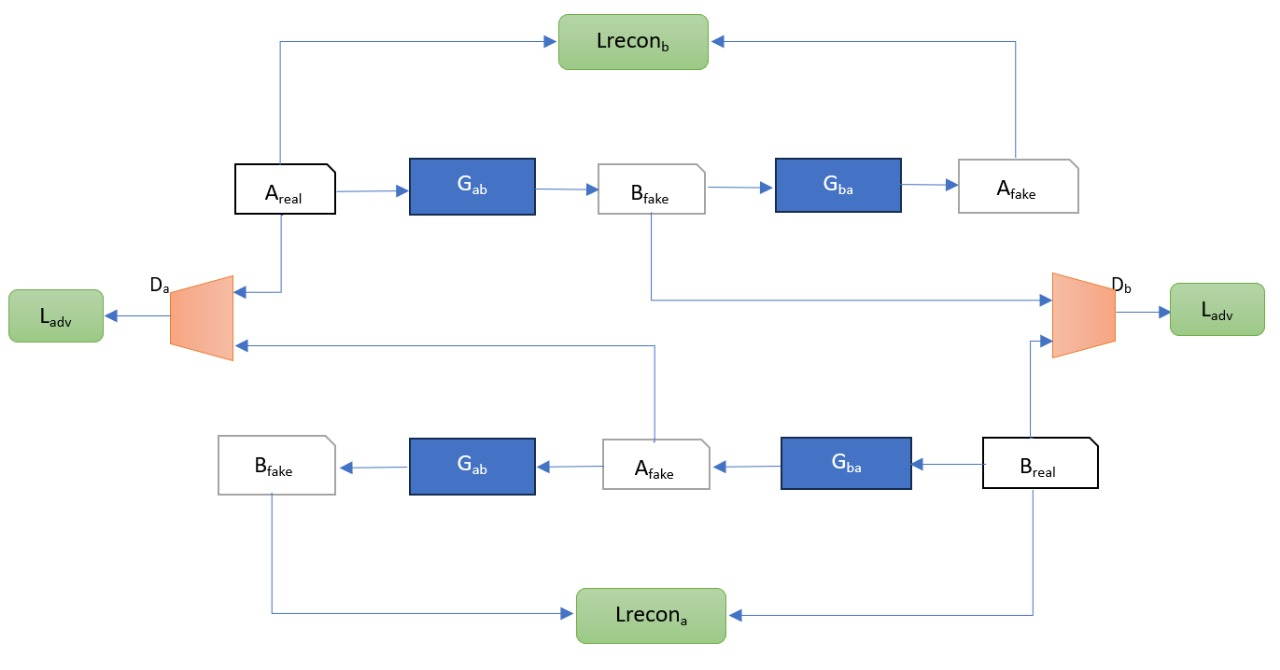
\includegraphics[scale = 0.5]{discoGAN}
  \caption{DiscoGAN Architecture}
  \label{fig:DiscoGAN}
\end{figure}

$A_{real}$ represents the real input image. It is passed through $G_{ab}$ which is a generator that converts image from domain A to B. This generates the fake image in domain B, $B_{fake}$. This is then passed through another generator $G_{ba}$ which converts it back to an imge from domain A.
This is labelled as $A_{fake}$. The fake image from each domain along with the real image in each domin is passed through a discriminator for each domain, $D_a$ and $D_b$ repectively. $L_{adv}$ represents the adversarial loss and is calculated between the real image and the fake image generated by the generator. 
\begin{equation}
\mathcal{L}_{\text{A}} = -\mathbb{E}_{A}[\log(D(A))] - \mathbb{E}_{B}[\log(1 - D(G_{ba}(B)))]
\end{equation}
\begin{equation}
\mathcal{L}_{\text{B}} = -\mathbb{E}_{B}[\log(D(B))] - \mathbb{E}_{A}[\log(1 - D(G_{ab}(A)))]
\end{equation}

The reconstruction loss is defined as the difference between the real image and the image retrieved after translating it to the other domain and back. The loss is generally calculated via mean squared loss or L2 norm. It is denoted as :
\newline
\begin{equation}
Lrecon_{b} = (A - G_{ba}(G_{ab}(A)))^{2}
\end{equation}
\begin{equation}
Lrecon_{a} = (B - G_{ab}(G_{ba}(B)))^{2}
\end{equation}

Each reconstruction loss is used to fine-tune their respective generators. 


This divergence in objectives makes DiscoGAN particularly well-suited for applications where understanding and exploiting cross-domain relationships are paramount, with potential uses spanning various domains, from style transfer to gait analysis.

 
\subsection{M-DiscoGAN}
M-DiscoGAN is a novel variation of the traditional DiscoGAN framework that introduces the Wasserstein Generative Adversarial Network (WGAN) loss to enhance its performance. In this modified architecture, instead of relying on the conventional adversarial loss, M-DiscoGAN leverages the WGAN loss to improve training stability and generate more realistic image-to-image translations. This combination of these loss functions enhances the overall quality of the generated outputs and fosters a more efficient training process, making M-discoGAN a promising model for various image translation tasks.

\begin{figure}[!h]
  \centering
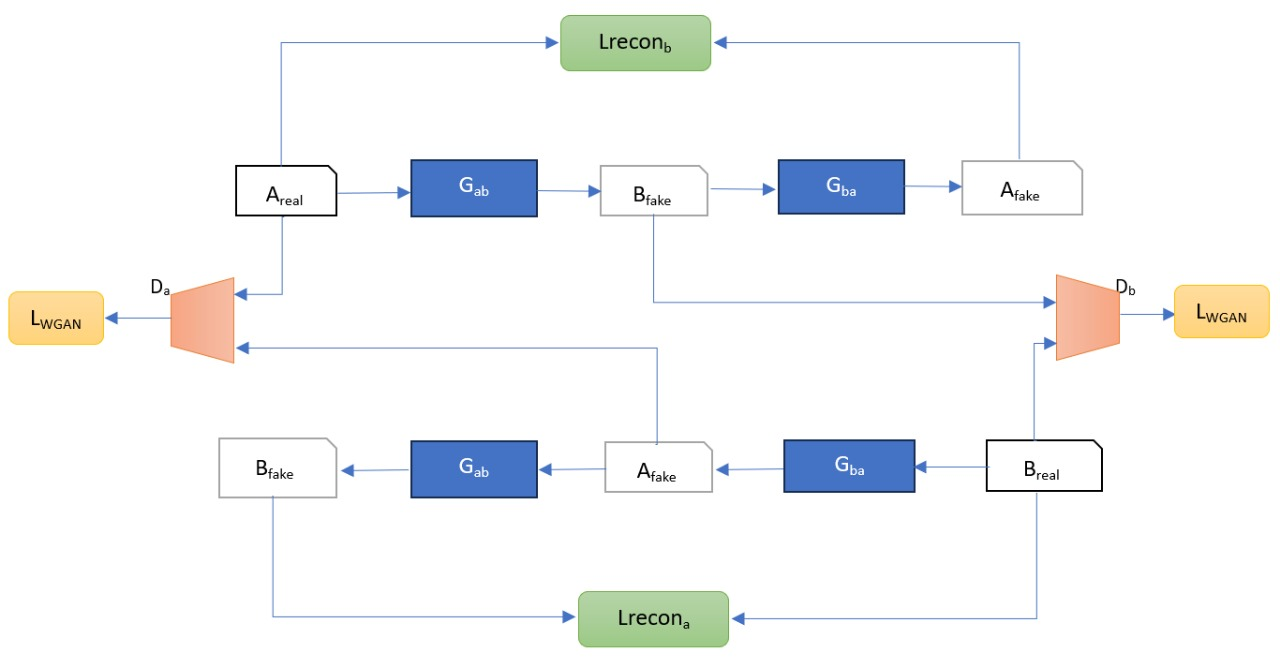
\includegraphics[scale = 0.5]{images/M-discoGAN.jpg}
  \caption{M-discoGAN Architecture}
  \label{fig:cycleWGAN}
\end{figure}

\clearpage
\subsection{GEI Images}

\begin{figure}[!h]
    \centering
    \begin{subfigure}{0.45\textwidth}
        \centering
        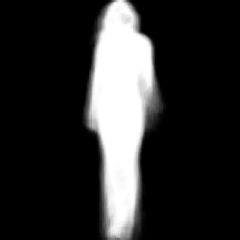
\includegraphics[width=0.8\textwidth]{walk-nm1.jpg}
        
        \label{fig:img1}
    \end{subfigure}
    \begin{subfigure}{0.45\textwidth}
        \centering
        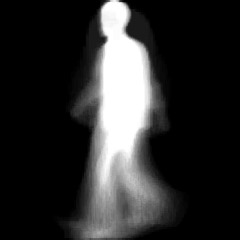
\includegraphics[width=0.8\textwidth]{walk-nm2.jpg}
        
        \label{fig:img2}
    \end{subfigure}
    \caption{GEI involving normal walk}
\end{figure}

\begin{figure}[!h]
    \centering
    \begin{subfigure}{0.45\textwidth}
        \centering
        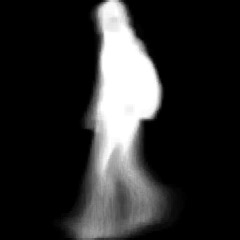
\includegraphics[width=0.8\textwidth]{walk-bg1.jpg}
        
        \label{fig:img1}
    \end{subfigure}
    \begin{subfigure}{0.45\textwidth}
        \centering
        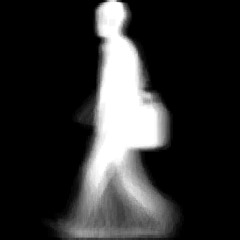
\includegraphics[width=0.8\textwidth]{walk-bg2.jpg}
        
        \label{fig:img2}
    \end{subfigure}
    \caption{GEI involving bags}
\end{figure}

\begin{figure}[!h]
    \centering
    \begin{subfigure}{0.45\textwidth}
        \centering
        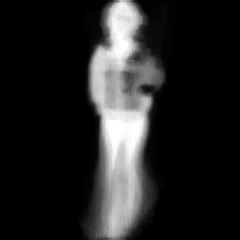
\includegraphics[width=0.8\textwidth]{walk-cl1.jpg}
        
        \label{fig:img1}
    \end{subfigure}
    \begin{subfigure}{0.45\textwidth}
        \centering
        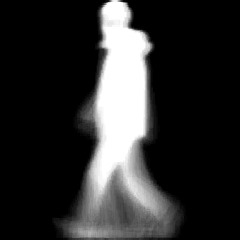
\includegraphics[width=0.8\textwidth]{walk-cl2.jpg}
        
        \label{fig:img2}
    \end{subfigure}
    \caption{GEI involving clothes}
\end{figure}
    
    % \begin{subfigure}[b]{0.4\textwidth}
    %     \centering
    %     \inc

\subsection{Gan architecture}
The heart of the proposed system lies in the application of Generative Adversarial Networks (GANs) for image-to-image translation. GANs consist of two key components: generators and discriminators. 
\begin{figure}[!h]
  \centering
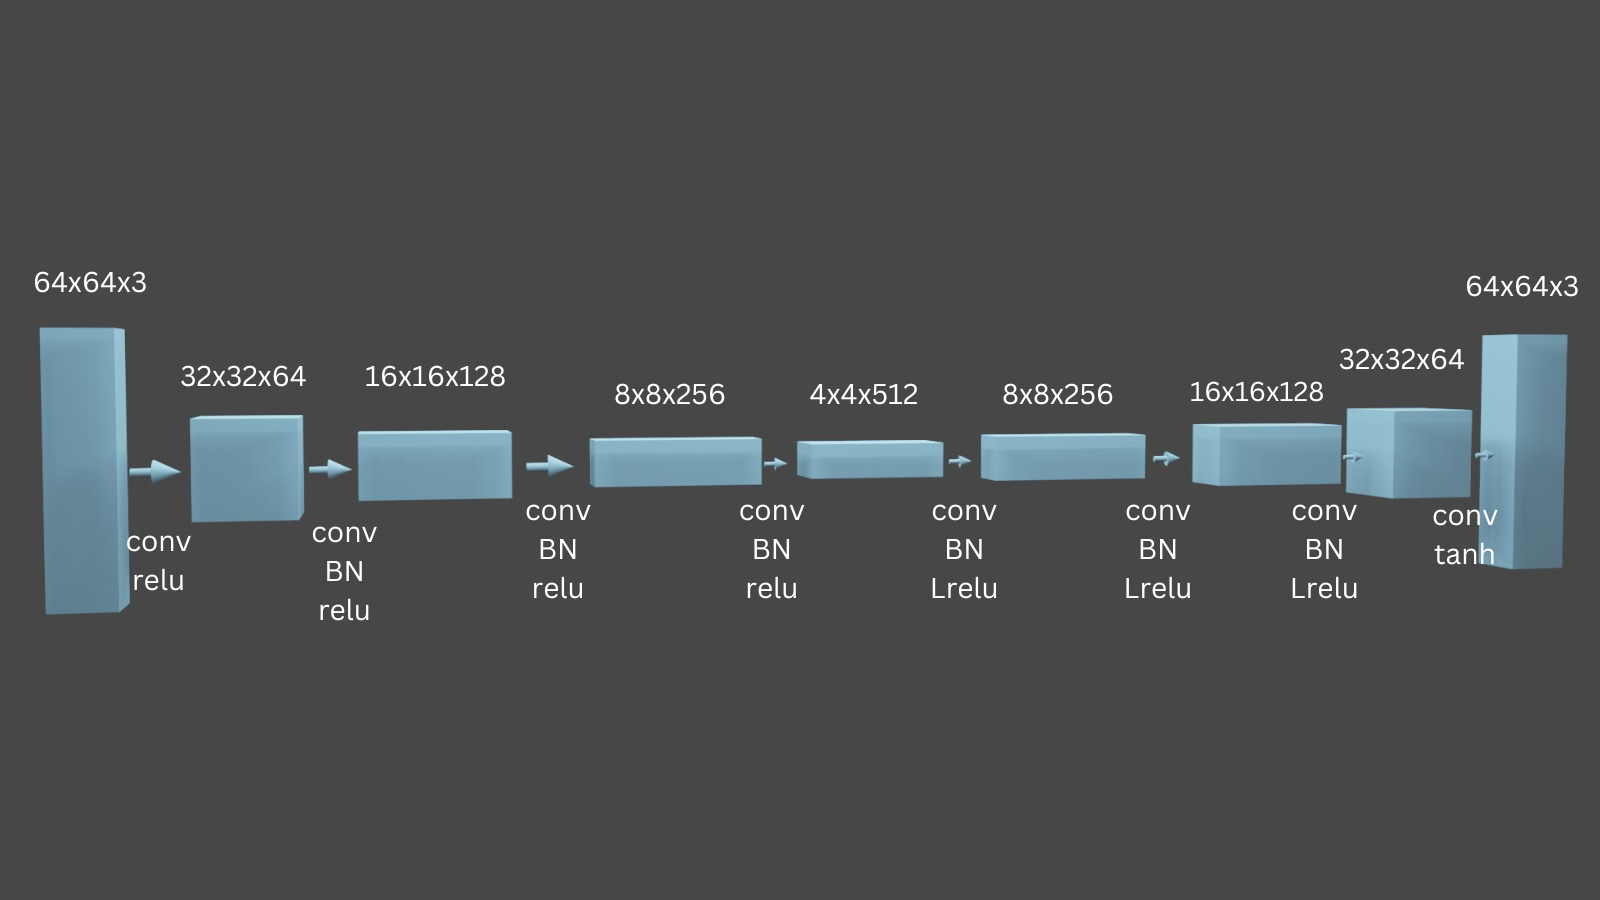
\includegraphics[scale = 0.35]{images/gen.png}
  \caption{Generator Architecture}
  \label{fig: Gen architecture}
\end{figure}
Generators aim to produce images that resemble a specific target domain, by performing downsampling and upsampling using layers convolution layers, batch norm, leaky Relu, Relu, and tanh functions. Discriminators evaluate these generated images, attempting to distinguish between real and generated GEIs.
\newline

In summary, the proposed system begins with frame-by-frame analysis, converts the individual frames to an overall GEIs and employs GAN-based image-to-image translation to remove covariate factors. By combining the three GAN structures and utilizing a voting classifier, the system optimizes the translation process, whose output is then fed into the CNN for an efficient person identification.
\clearpage
\section{Timeline}

\begin{figure}[htb!]
  \centering
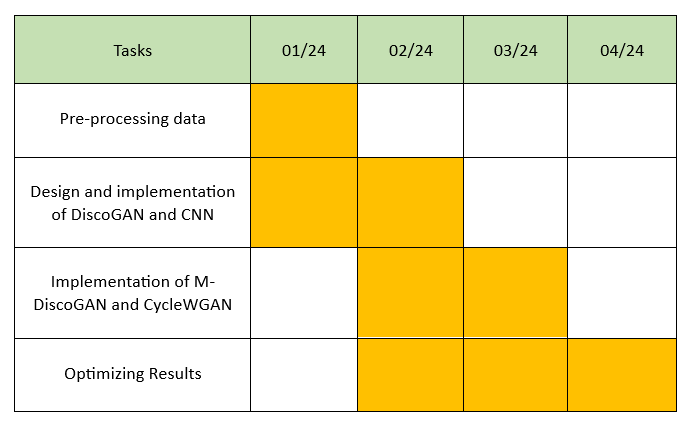
\includegraphics[scale = 0.85]{timeline-chart.png}
  \caption{Project Timeline}
  \label{fig:cycleWGAN}
\end{figure}



\begin{thebibliography}{99}
  \bibliographystyle{plain}

\bibitem[1] {zou2020} Zou, Q., Wang, Y., Wang, Q., Zhao, Y., Li, Q. (2020). Deep learning-based gait recognition using smartphones in the wild. {\em IEEE Transactions on Information Forensics and Security, 15, 3197-3212.}


\bibitem[2] {manssor2021}Manssor, S. A., Sun, S., Elhassan, M. A. (2021). Real-time human recognition at night via integrated face and gait recognition technologies. Sensors, 21(13), 4323.

\bibitem [3]{huynh2020}Huynh-The, T., Hua, C. H., Tu, N. A., Kim, D. S. (2020). Learning 3D spatiotemporal gait feature by convolutional network for person identification. {\em Neurocomputing, 397, 192-202.}

\bibitem [4]{asif2022}Asif, M., Tiwana, M. I., Khan, U. S., Ahmad, M. W., Qureshi, W. S., Iqbal, J. (2022). Human gait recognition subject to different covariate factors in a multi-view environment. {\em Results in Engineering, 15, 100556.}

\bibitem [5]{vasudevan2023} Vasudevan, P., Mattins, R. F., Srivarshan, S., Narayanan, A., Wadhwani, G., Parvathi, R., Maheswari, R. (2023). Gait image classification using Deep Learning Models for medical diagnosis.{\em CMC-COMPUTERS MATERIALS CONTINUA, 74(3), 6039-6063}

\bibitem[6]{wen2022}Wen, J., Shen, Y., Yang, J. (2022). Multi-view gait recognition based on generative adversarial network. {\em Neural Processing Letters, 54(3), 1855-1877.}

\bibitem[7]{khan2023}Khan, M. A., Arshad, H., Khan, W. Z., Alhaisoni, M., Tariq, U., Hussein, H. S., ... Elashry, A. (2023). HGRBOL2: human gait recognition for biometric application using Bayesian optimization and extreme learning machine.{\em Future Generation Computer Systems, 143, 337-348.}

\bibitem[8]{liao2020}Liao, R., Yu, S., An, W., Huang, Y. (2020). A model-based gait recognition method with body pose and human prior knowledge. {\em Pattern Recognition, 98, 107069.}

\bibitem[9]{kim2017}Kim, T., Cha, M., Kim, H., Lee, J. K., Kim, J. (2017, July). Learning to discover cross-domain relations with generative adversarial networks. {\em In International conference on machine learning (pp. 1857-1865). PMLR.}

\bibitem[10]{arjovsky2017} Arjovsky, M., Chintala, S., Bottou, L. (2017, July). Wasserstein generative adversarial networks. {\em In International conference on machine learning (pp. 214-223). PMLR.}

\bibitem[11]{hu2021} Hu, W., Li, M.,  Ju, X. (2021). {\em Improved CycleGAN for image-to-image translation.}

\bibitem[12]{zhu2017}Zhu, J. Y., Park, T., Isola, P.,  Efros, A. A. (2017). Unpaired image-to-image translation using cycle-consistent adversarial networks.{\em In Proceedings of the IEEE international conference on computer vision (pp. 2223-2232).}

\bibitem[13] {alsaggaf2021}Alsaggaf, W. A., Mehmood, I., Khairullah, E. F., Alhuraiji, S., Sabir, M. F. S., Alghamdi, A. S., ... Ahmed, A. (2021). A smart surveillance system for uncooperative gait recognition using cycle consistent generative adversarial networks (CCGANs). {\em Computational Intelligence and Neuroscience, 2021.}

\end{thebibliography}



	
\end{document}
